\documentclass{ucl_thesis}
% LaTeX source code based on an example by Gabriel Brostow,
% which is based on earlier work of Simon Prince, Macolm Reynolds
% and Mark Herbster.

%twoside for double page printing
\usepackage{graphics}
\usepackage{graphicx}
\usepackage{color}
\usepackage{verbatim}
\usepackage{algorithm}
\usepackage{algorithmic}
\newcommand{\theHalgorithm}{\arabic{algorithm}}
\usepackage{listings}
\usepackage{amsmath}
% Uncomment this to activate the TikZ library, which is useful for fancy block-diagrams.
%    \usepackage{tikz}
%    \usetikzlibrary{positioning,arrows,shapes.misc}
\usepackage{multirow}
%\numberwithin{algorithm}{chapter}
%\usepackage{epsf}
\usepackage{fancyvrb}
% Uncomment this package to enable internal-linking:
%\usepackage{hyperref}


%%%%%%%%%%%%%%%%% TODO %%%%%%%%%%%%%%%%% 
% - clean up example report code


%%%%%%%%%%%%%%%%% COMMANDS %%%%%%%%%%%%%%%%% 
\newcommand{\vect}[1]{\boldsymbol{#1}}
\newcommand{\figref}[1]{(Fig. \ref{#1})}

\def\etal{{et~al.}}

% I also like these, but didn't have occasion to use them below:
\def\ie{{\it i.e.,\ }}
\def\etc{{\it etc.,\ }}
\def\eg{{\it e.g.,\ }}
\def\vs{{\it vs.\ }}


%\renewcommand{\baselinestretch}{1.5}
%\renewcommand{\bibname}{References}


%%%%%%%%%%%%%%%%% TITLE PAGE %%%%%%%%%%%%%%%%% 

% worktitle
\title{Constructing the concave hull of an outdoor scene
       using visibility traces of points and edges}

\author{Martijn Frederik Wouter van der Veen}
\def \supervisor {Gabriel J. Brostow}

\date{September 2012}

\begin{document}
\bibliographystyle{abbrv}
\maketitle
\numberwithin{algorithm}{chapter}
\setcounter{page}{1}
\pagenumbering{roman}
\pagestyle{plain}

% Notice how the star "*" is used throughout LaTex to modify the normal behavior. For example, \section* instead of \section 
% tells LaTex NOT to number this section.



%%%%%%%%%%%%%%%%% INTRODUCTION PAGES %%%%%%%%%%%%%%%%% 

\newpage
\section*{Abstract}
%Geometry reconstruction has been an important but challenging field of research within computer vision. Many approaches rely on extracting certain features (silhouettes, interest points, similar coloured pixels) from images, and are inherently dependent on the ability to find reliable features on all objects. Objects not rich in features or objects with non-Lambertian properties result in poor reconstructions. However, detection failures can provide useful clues as well. In this thesis, we propose an approach based on both visibility of detected features \emph{and} occlusion of features detected in other images. The approach aims at finding and reconstructing objects \emph{indirectly} by noticing the absence of expected features, without relying on detection of any cues on the objects theirselves.

The suggested approach is tested on new datasets containing footage of low-textured and reflective objects. Given enough view points and texture on background objects, the developed and implemented method is able to reconstruct both low-textured and reflective objects. Results are compared to a state-of-the-art dense stereo reconstruction and found to perform better on reflective and big low-textured objects. 



\newpage
\section*{Acknowledgements}

%\setcounter{tocdepth}{2}
\tableofcontents
\listoffigures
%\listoftables
\listofalgorithms
\newpage

%\clearpage
%
%\begin{center}
%\textbf{To whomever}
%\end{center}

\setcounter{page}{1}
\pagenumbering{arabic}
\pagestyle{plain}



%%%%%%%%%%%%%%%%% CONTENT: INTRODUCTION %%%%%%%%%%%%%%%%% 

\chapter{Introduction}
\label{introduction}
%%% INTRODUCTION:
%  a. Motivation

The understanding of physical scenes by machines has been of great interest for researchers over the last couple of decades. Being able to construct the three dimensional shape of objects in a scene can be very helpful in this task. Based on the observation that, for humans, visual clues seem quite useful for understanding the structure of their environment, it is not surprising that researchers in the field of computer vision have put a great deal of effort in trying to build algorithms that construct 3D models out of images. Being able to reconstruct geometry allows for new applications. On a practical level, for example, it allows for easy creation of 3D models for usage in modelling design, computer games and even 3D printing. In addition, geometry reconstruction as an intermediate step opens the door to further processing in advanced street scene understanding, advanced geometry-aware rendering of new or editing of existing footage (such as changing lighting or virtually moving objects in the scene), navigational tasks in robotic systems, and augmented reality applications\footnote{One could even state that geometry reconstruction could be seen as an intermediate feature in advanced computer vision, much in the same way as edge detection is used extensively as a feature in more advanced image processing algorithms.}. Increasing computer power, cheap and omnipresent cameras, and recent developments in the field of computer vision and learning all help making these exciting applications a reality.

%  b. Problem statement
There has been published a great amount of research on geometry reconstruction. A variety of approaches has been proposed, each with their own advantages and disadvantages. Most, if not all, of the approaches seem to be based on one or more visual clues that are relatively easy to find automatically, such as silhouettes, corner points or similarly coloured pixels in images. Different visual clues call for various requirements in the input images, resulting in successes and failures specific for the chosen approach. Current approaches often rely on the ability to detect features such as silhouettes or distinctive corner points on \emph{all} geometry, resulting in bad results for objects where the specific features are less present.

However, detected features are not the only pieces of information that can be used for geometry reconstruction; failure of detection can provide useful information too. Detection failures can be detected by using information from features detected in other parts of the data (\eg other images). In particular, the absence of features in images were they would have been expected due to detection in images taken from surrounding camera poses may indicate the existence of another object. Although this observation might seem obvious, it has not got a lot of attention in the computer vision literature. Bad matches or the absence of features have mostly been threated as outliers or as an indication for not using certain data in a particular step in the reconstruction; it has seldomly been used actively for reconstructing geometry\footnote{It is almost as if researchers are afraid of negative information.}. Often camera poses are thrown away after triangulating the feature locations, continuing with the positive information (features) only. Intuitively, this seems like throwing away useful information. It is this intuition that motivates the approach taken in this thesis.

In this thesis, a framework is proposed that uses both \emph{visibility} (detected features) and \emph{occlusion} (undetected but expected features) in order to find, and reconstruct, objects not rich in features. The proposed method uses features detected on other parts of the scene to find objects difficult to detect directly. Based on the visibility and occlusion information of features from given observation locations, space is `carved' in a probabilistic way. The method has been tested on a variety of outdoor scenes and, given enough detected features on objects in the background, gives high probabilities for regions containing objects difficult to detect with widely-used alternative methods. While space-carving based on silhouettes has difficulties with high-textured and complex outdoor scenes, and multi-view stereo is challenged by low-textured and reflective objects, the suggested method targets at scenes containing both and aims at combining strong properties of both methods.

% UCL website wants this. bit informal
In the course of the project that resulted in this report, most of the time has been used for the practical implementation and evaluation, in addition to a comprehensive literature review and documentation. Various software libraries have been tested and used to develop not only the method described here, but also several visualisation tools helpful for the visual thinking process necessary for developing geometry algorithms. Since our results are inherently three-dimensional and this report is not, the reader is encouraged to view the supplemented digital material - either using the provided tools or pre-made videos - alongside reading the report.





%%%%%%%%%%%%%%%%% CONTENT: BACKGROUND %%%%%%%%%%%%%%%%% 
\chapter{Background}
\label{background}
%%% background

%  a. introduction

Geometry reconstruction has drawn a lot of attention in the computer vision community (\Hartley2003, \Seitz2006, and \Prince2012). The goal is to reconstruct the three dimensional structure of a particular scene given the data, usually multiple images (Multi-View Stereo). The images can come from different cameras (unordered set), or from the same camera (sequence) that potentially has been moved around. For many algorithms the relative locations from the cameras are required. They are either obtained by calibration between the different cameras or images (\eg by some identifiable pattern visible in all the images, or measured using external sensors), or estimated based on features naturally occurring in the images. When the positions are known, all the pixels in an image are known to be a projection from a particular point somewhere on a line through the camera centre and the pixel on the image plane, with the location of the point on the line being the only ambiguity. The next task now is to estimate the geometry of the scene pictured in those images, given this ambiguous information. Different approaches exist to tackle this problem, of which we will discuss four categories: layers (Section \ref{layers}), space carving (Section \ref{carving}), structure from motion (Section \ref{sfm}), and Multi-View Stereo using Depth Maps (Section \ref{mvs}). We like to note, however, that often multiple approaches are combined and overlap exist. Not all the techniques being discussed are directly relevant to the proposed algorithm, but they give a sense of the variety of approaches being published and try to give a general overview of the geometry reconstruction research literature.


%  b. Layers in video
\pagebreak
\section{Layers in Video}  \label{layers}
One of the earlier, and in some aspects simpler, attempts to represent geometry in images is the use of layers. Images are assumed to be a composition of multiple, possibly overlapping, surfaces that can move relative to one another from frame to frame in a sequence. Objects pictured in images can be at different distances to the camera, resulting in overlapping surfaces when projected onto an image (\ie captured). Successfully identifying coherent surfaces, including their mutual occlusions and movements from one frame to another, allows for a scene representation consisting of \emph{layers}. Such a representation usually consists of one background layer plus one or more foreground layers representing objects moving in front of the background layer.

As one of the first to suggest representing sequences of images with layers, \Wang1994 decomposed images into `motion layers' by analysing the motion of extracted segments in the subsequent images using optical flow. Segments with similar motions are combined, and grown and depth-ordered by tracking them over the sequence, resulting in more extensive layers. The layers can then be used in combination with estimated simple motion models to reconstruct the sequence in a memory-efficient way. Multiple extensions on this scheme exist. For example, \Jojic2001 subdivided layers into flexible sprites that can vary their shapes according to a probabilistic model. The sprites and their probabilistic models are learned using the Expectation Maximisation algorithm on a representation consisting of one appearance and one mask pixel vector per sprite. Theoretically, the unsupervised EM learning approach even allows for finding sprites in related but unordered photo collections. Another approach, suggested by \Smith2004, is to extract and track edges over the sequence in order. Motion models are then fit to the edges using the EM algorithm. The edges, which form a better criterion for segment borders than the locally-smoothed optical flow vector field, are used to find a good segmentation of the frames and segments with similar motion models are again merged, thereby resulting in layers.

Although layered representations do have the notion of depth-ordering - and thus occlusion - they do not aim at recovering the exact depth of the layers, and inherently do not reconstruct three-dimensional geometry. In the next section, we move on to three alternative approaches that aim at true geometry recovery.

Layers are relevant for the current work because initially the intuition was raised that footage of an outdoor scene can be segmented into layers by tracking feature points and noticing when occlusions happen. However, for these feature points we can estimate the three-dimensional location by using Structure from Motion techniques (Section \ref{sfm}), allowing to reconstruct more than relative order. Hence, the step from layers to real three-dimensional reconstruction was made and the proposed method as described in Section \ref{method} originated.


%  c. Carving
\pagebreak
\section{Space carving}  \label{carving}
While layers in videos try to represent geometry by their projections onto the image planes, thereby ignoring the original three-dimensional geometrical shapes, space carving aims at estimating the actual surface of objects in a scene. To reconstruct 3D from flat projections, space carving assumes the camera poses are known, \ie we have calibrated cameras. The poses are either known due to explicit calibration (using a calibration object or external sensor), or estimated based on the natural content of the images.

Usually, space carving is based on finding silhouettes \cite{Hartley2003, Matusik2000}, thus segmenting each of the images into a binary background and foreground `layer' or mask. These techniques are also known as Structure from Silhouettes. The pixels in the images are known to be projections of points somewhere on lines from the camera centres passing through the pixels, but the locations on the lines (\ie depths) are unknown. Space carving based on silhouettes\footnote{Part of the literature reserves the term Space Carving for space carving based on photo-consistency as described later on; here, it is used for both photo-consistency and silhouette-based space carving iteratively refining a model represented by a voxel grid.}. does not estimate this depth; instead, it uses the background-foreground masks to categorise each line as either intersecting with an object, or not. The foreground mask therefore represents a cone of space in which the projected object must lie, at unknown distance. 

For reconstruction, usually a 3D volume is chosen that lies in between the camera poses, and the volume is discretised and represented as a \emph{voxel grid} - although polygonal representations have been proposed too. Space carving starts with all the voxels marked as `object'. For each camera pose, all the voxels are projected onto the image plane. Voxels projecting to pixels not set as foreground (\ie onto the background mask) are set to `non-object', finally resulting in the intersection of cones in which the object must lie (see Figure \ref{fig:carving}). This intersection is called \emph{visual hull} or \emph{convex hull}. It can be used as the final reconstruction, or used as a useful prior for further processing as the maximum (convex) boundary in which search can continue.

\begin{figure}[htb!]
 \centering
 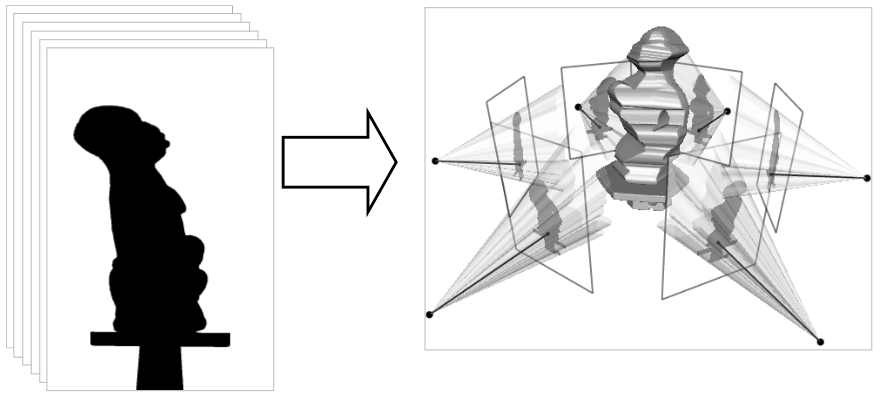
\includegraphics[width=1.0\textwidth]{img/carving}
 \caption{Carving using silhouettes. Image taken from `How to prepare and deliver a presentation' [ppt] by R. Cipolla, who adopted it from unknown source}
 \label{fig:carving}
\end{figure}

Segmenting images in foreground and background masks can be accomplished by a simple threshold, or by learning more advanced colour models for both. This can be user-guided or automated. For example, \Campbell2007 automatically learned foreground colour models using pixels at the centre of the images (requiring the user making the footage to fixate at the object of interest) and background colour models using pixels near the image corners. The initial colour models are used together with the calibrated camera poses to make an initial binary segmentation in a voxel grid. The segmentation is then used to refine the colour models, and the process is repeated until the solution converges. As is common in algorithms involving voxel grid representations, \Campbell2007 use a Markov Random Field (MRF) prior for the segmentation step, promoting local smoothness for obtaining a global solution. A min-cut/max-flow graph-cut algorithm like the one presented by \Boykov2004 is used to find the solution. This process is also known as regularisation.

Using more pictures in the space carving approach will give better approximations. However, concavities are not visible from silhouettes, so they will not turn up in the final reconstruction. The acquired visual hull therefore is only a broad approximation of the object's surface. Space carving is very suitable to do on a turn-table, for which the background model is known and also the relative camera poses are known due to controlled turn-table rotation. However, a turn-table is only feasible for objects small enough to put on the device. Placing a green screen behind objects is also a possibility, resulting in the same easy silhouette segmentation. Green screens have their limits too, making it an unsuitable remedy for outdoor scenes, where the background often is not controllable. Furthermore, space carving is not suitable for dynamic scenes. As a last disadvantage, multiple objects are not easy recognisable in a single silhouette and will result in ghosting objects \cite{Guan2007}.

Extensions have been proposed to overcome the limited applicability of carving based on silhouettes. For example, \GuanOld added time-dependent Bayesian probability to the voxel variables, allowing space carving to be used in dynamic scenes. In their representation, voxels represent probabilities on occlusions before and after the voxel on a line passing through the centres of a set of calibrated cameras, filming from fixed locations. Using time-dependencies, their algorithm is able to follow dynamic objects over time, \eg a human walking through a temple. To find silhouettes, a per-pixel Gaussian background colour model is made for every camera before the dynamic object enters the scene. The estimates of the silhouettes are used as a prior for the next time frame, allowing to spot the object moving behind static occluders. When the object moves extensively through the scene, static occluders will turn up when they occlude the object. Even concavities in static occluders can be detected if an object moves, in fact allowing to carve away all human reachable locations by walking through the scene. In a later publication, \Guan2008 extended their algorithm to detect and label multiple dynamic objects. Each time a new, unknown silhouette (that differs enough from the colour models learned so far) enters the scene, a new appearance colour model is learned. Although the algorithm only works with fixed cameras and dynamic objects, it does have notion of visibility and occlusion.

An alternative to space carving with silhouettes is space carving based on photo-consistency, as introduced by \SeitzOld. Hereby, voxels are projected onto all image planes that are able to see the voxel according to the current voxel grid. The set of pixels a voxel projects to are then checked for photo-consistency in compliance with a reflectance model (BRDF). The photo-consistency check returns the probability of this set of pixel colours originating from the same surface point. For a low photo-consistency score, it is unlikely that this voxel is part of a solid object, and so it is carved away. The process continues until all the remaining uncarved voxels have a high photo-consistency. Although results look promising, the algorithm has some problems with low-textured (\ie uniformly coloured) objects and objects with repetitive textures. Furthermore, the method does not scale very well to bigger environments with lots of same coloured objects, and assumes Lambertian surfaces for all objects. In practise, pixels usually have no unique colour and reflective objects are not uncommon.

% TODO: improve
As a last example in the space carving literature, we discuss the work by \Hernandez2007, who further explored the concept of visibility using the photo-consistency criterion. The algorithm introduced by \SeitzOld is extended to include a probabilistic voxel grid: voxels are not carved one by one, but assigned the photo-consistency probability for being part of the surface of an object \footnote{In fact, a fast depth-map (Section \ref{mvs}) computation is done and photo-consistency is calculated only for locations with 3D points nearby}. A second voxel grid represents the visibility evidence, containing probabilities of voxels being visible by at least one camera. This will give a penalty to voxels that are presumed not to be visible from any camera, and thus not part of the surface of an object. As a final step, graph-cut is used to combine the photo-consistency and visibility voxel grids, obtaining the assumed surface. Note that occlusion is being used, but only to exclude voxels inside objects, not for refining the shape itself.


%  d. Structure from Motion
\section{Structure from Motion}  \label{sfm}
Geometry reconstruction usually involves measurements in the form of images, that is, flat projections of the three-dimensional world at specific locations (and times). If these locations are known, the process of reconstructing the original scene becomes easier. Therefore, much effort has been put in reliable pose estimation. Structure from Motion, as described extensively by \Hartley2003, tries to accomplish this. Structure from Motion (SfM) uses natural features in images in order to estimate the relative translation and rotation between the camera poses of different images. It is based on the intuition that moving your head (motion) and noticing differences of the different views allows for a rough estimation of objects and distances (structure) in a scene.

For SfM techniques, the camera poses are unknown a priori and need to be estimated based for a set of given images. As a first stage, features such as interest (corner) points are found in all images. One of the most popular features is SIFT, as introduced by \Lowe2004. SIFT features are found by searching for maxima in scale-space, constructed with Derivative of Gaussian filters. For the detected locations, a unique SIFT descriptor is constructed based on a histogram of gradient directions of points nearby. SIFT features are scale and rotation invariant and partially intensity and contrast change invariant. Alternative features can be used too, as long as they can be matched uniquely between images. In the second step, the interest points are matched between images using their descriptor. Using the matching pairs between images allows for estimating the relative transformation from one camera to another by satisfying projective geometry constraints (\Prince2012, Ch15-16, \Hartley2003, Ch10-12). For every image pair with estimated transformation, 3D locations of matched interest points can now be estimated by triangulation (Fig. \ref{fig:sfm_triangulate}). The depth ambiguity for \emph{some points} is now eliminated in each image. The image pair point clouds - possibly containing feature points seen in multiple image pairs - can be combined using Bundle Adjustment (\eg, \Wu2011, \Hartley2003, Ch18), which minimises noise and estimation errors in point and camera pose locations and obtains a global solution. The result is a \emph{sparse point cloud} (Fig. \ref{fig:sfm_sparsepointcloud}), camera models (including pose), plus visibility lists with camera-points pairs.
As an example of using alternative features, \Chandraker2009 developed a Structure from Motion system based on lines, arguing that indoor environments and scenes containing much human-made objects usually lack distinctive feature points, but a rich of straight lines. Line geometry constraints are used to estimate camera translation and rotation in a similar way as in the case points are used.

\begin{figure}[htb!]
 \centering
 \subfigure[3D point location estimation by triangulating two matched feature points in a pair of images]{
  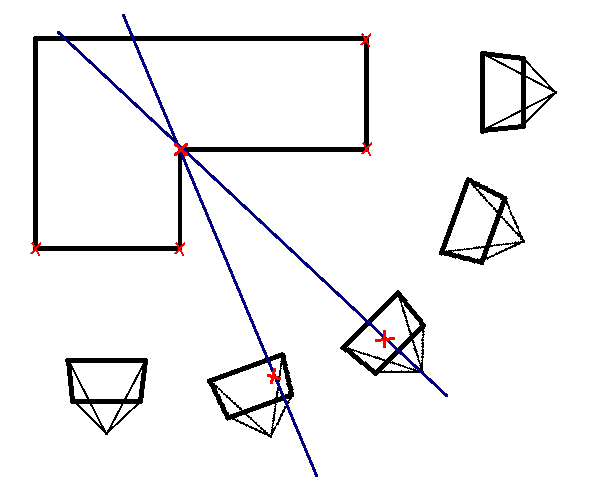
\includegraphics[width=0.45\textwidth]{img/sfm_triangulate}
  \label{fig:sfm_triangulate}
 }
 \subfigure[Sparse point cloud. Image taken from http://grail.cs.washington.edu/rome/dense.html (1st of March 2012)]{
  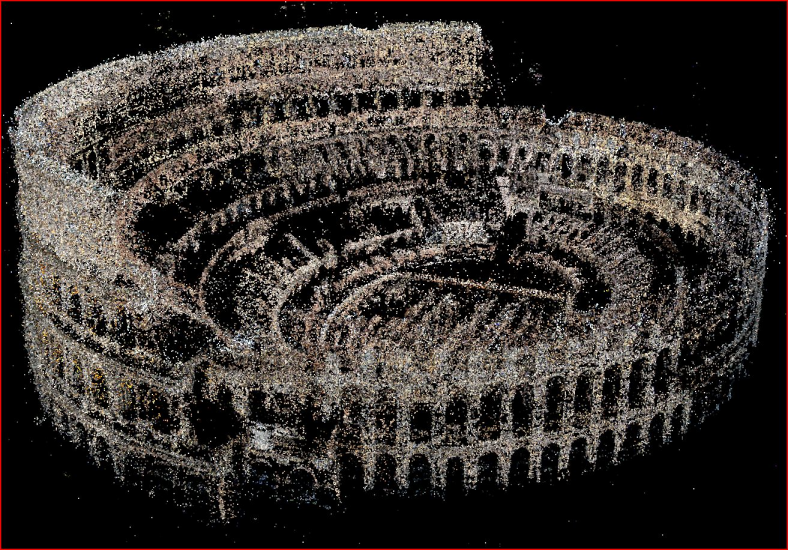
\includegraphics[width=0.45\textwidth]{img/sfm_sparsepointcloud}
          \label{fig:sfm_sparsepointcloud}
 }
 \caption{Structure from Motion}
 \label{fig:sfm}
\end{figure}

After reconstructing both the sparse point cloud and camera poses, usually one of the two is thrown away and the other is used in a subsequent step. Given the sparse point cloud, one can attempt to reconstruct geometry based on the sparse, but reliable points. Different techniques have been used \cite{Seitz2006}. One simple way of doing this is fitting a polygon mesh to the point cloud. More advanced smooth surface fitting is also possible, as has been done for example by Izadi~\etal~\cite{Izadi2011}, but it eliminates strong edges and flat surfaces which are overrepresented in real scenes. Another method is fitting primitive shapes like planes and lines to the point cloud, which works well in human-made environments, but not so well in outdoor scenes. In all cases, assumptions are made on possible interpolation between points close to each other, and lack of texture results in gaps and sometimes missing objects in the reconstruction. In practise, sparse point clouds are rarely used for surface reconstruction. More often, the camera poses are kept and used in combination with the original images using a subsequent algorithm (\eg space carving (Section \ref{carving}) or depth maps (Section \ref{mvs})), obtaining a more dense representation before surface reconstruction is attempted.
% TODO: photo tourism here as possible application of sparse point cloud only


%     - Visibility and Occlusion 
% TODO: move to end MVS? NO: makes sense here
%       (depth maps less clear if they have lists of visibility; plus most papers here are about sparse point clouds)
\subsection{Visibility and Occlusion}
An important observation that did not got a lot of attention in the literature is the fact that the visibility of the points over time (\ie over the image sequence) can not only help selecting and fine-tuning points in either sparse or dense point clouds (as noted in the survey of Seitz~\etal~\cite{Seitz2006} and used in \cite{Merrell2007, Hernandez2007}), but also directly used for surface reconstruction. In other words: occlusion rarely has an essential role in geometry reconstruction. However, visibility tracks over time can help both finding empty space (because we can see points at a certain location from a certain location) and finding occluder objects (because we lost track of a point for a while). Structure from Motion - in addition to pose estimation - therefore does not only deliver sparse points on surfaces, but also gives information about the occupancy state of space between the camera poses and reconstructed sparse points, without the need to find any visual clues at that locations. This observation has an essential role in the proposed approach (Section \ref{method}).

% TODO: improve?
Despite the scarcity of occlusion applications, recently there have been some attempts worth a brief discussion. For example, \ZachOld extent the structure from motion pipeline by an outlier check by using `missing correspondences'. Their method collects triplets of images connected by fair amounts of correspondences. Two of the images are used to triangulate the (sparse) correspondences which are projected into the third image. A probabilistic measure based on the number of found and missing correspondence points in the third image determines whether to discard the third image as a match or not. \Pan2009 propose geometry reconstruction (called ProFORMA) of single, well-textured, objects filmed with a fixed-position camera by calculating a sparse point cloud, converting the point cloud into a mesh using Delaunay tetrahedralisation, and carving away tetrahedra who violate visibility constraints. The carving consists of using intersections of rays from camera poses to points to determine - probabilistically - whether to carve away a intersected tetrahedra, finally obtaining a surface mesh. \Lovi2010 independently developed an almost identical system (called free-space carving) that can be used on more complicated scenes. Both methods use positive visibility information to carve away tetrahedra; however, negative occlusion information is not being used as tetrahedra are assumed to be occupied by default. Furthermore, the tetrahedralisation is based on triangulated feature points, requiring texture to be omnipresent and determinative for quality and resolution of reconstructed models.
Recently \Mcllroy2011 (2011) explored the possible use of both visibility and occlusion information with the aim of constructing high-level scene structure. In their approach, every (sparse) point is assigned a discretised `view sphere' whereby every solid angle bin saves the distance to the furthest camera within the solid angle that detected the point, plus the distance to the closest camera that did not detect the point. Using the view spheres primitives like planes and spheres are fitted to obtain probable locations of scene structure. However, results are shown for simple and well-textured scenes only, modelled by simple planes. Furthermore, since camera poses are used for the fitting, one needs to move extensively through the scene to provide the algorithm with enough camera poses. In contrary, the proposed method (Section \ref{method}) focusses not on the specific camera and point locations but on the rays in between, and thence indirectly finds low-textured and reflective objects using both visibility and occlusion information. In addition, a probabilistic voxel grid is used for discretisation allowing more general shape reconstruction, the implementation is tested on complex real-world scenes, and compared to state-of-the-art Multi-View Stereo results.

%  e. Multi-View Stereo using Depth Maps
\section{Multi-View Stereo using Depth Maps}  \label{mvs}
As a last category of geometry reconstruction methods, we will discuss reconstruction based on dense depth maps, often called stereoscopic. Usually, two steps are involved. In the first step, pairs or bigger sets of images are combined to form dense depth maps. The second step consists of carefully combining the depth maps in order to reconstruct scene geometry globally, for instance - as with SfM - by using bundle adjustment \cite{Wu2011}. Where space carving is mostly defined in scene-space by re-projecting voxel centres onto image planes, multi-view stereo (MVS) using depth maps applies its photo-consistency measure in image-space by comparing pixels \cite{Seitz2006}. Furthermore, as do structure from motion techniques, MVS using depth maps tries to estimate the depth of pixels explicitly. Depth maps, however, try to estimate this depth for every pixel, giving a dense depth or disparity map. However, estimating the depth for every pixel makes it necessary to match with less confidence than possible with SfM points, which can rely on stable and easy comparable feature points such as SIFT. Finally, combining the dense depth maps results in a \emph{dense point cloud}. We will now look into two different ways of creating the depth maps.

%     - active lighting
\subsection{Active lighting}
High precision in solving the depth ambiguity can be reached by actively illuminating part of the scene and searching for the illuminated part in images being taken. Depth map techniques recently received increased interest due to affordable active lighting sensors such as Kinect \cite{Izadi2011} reaching the commercial market, making depth vision suitable for a wider audience, but active lighting systems have been out there for a while. The illumination can consist of some fixed pattern (such as used by the Kinect and exploited by \Izadi2011), a sequence of different patterns (structured light), or a single (laser) point or line that moves over the surface (either for triangulation or time-of-flight). For example, a laser range-finder can be used to accurately map an environment by sending bright laser pulses and measuring travel times. \Huang2000 released a database containing range images obtained this way, together with a statistical analysis of natural depths in images. Although pattern-based devices like Kinect are becoming affordable, their active lighting patterns are weak and hence only suitable for indoor scenes. In general, accurate active lighting devices are less affordable and less practical than omnipresent cheap cameras. Therefore, much research effort has been put into passive depth vision based on regular images pairs.

%     - automated (depth vision)
\subsection{Passive depth vision}

\begin{figure}[htb!]
 \centering
 \subfigure{
  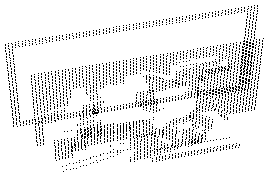
\includegraphics[width=0.45\textwidth]{img/depthmap1}
  \label{fig:depthmap1}
 }
 \subfigure{
  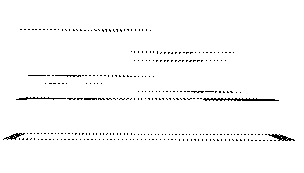
\includegraphics[width=0.45\textwidth]{img/depthmap2}
  \label{fig:depthmap2}
 }
 \caption{Two views of a depth map with few discretised depths, created by graph-cut algorithm. Image taken from own second years project, bachelor artificial intelligence, University of Amsterdam}
 \label{fig:depthmap_layer}
\end{figure}

If one would know, for every pixel in an image, the particular pixel displaying the same point in scene-space in a second image, the relative displacement allows for calculating the distance between that point in space and the camera (\cite{Prince2012}, Ch.14). The depth is estimated by triangulation using displacement and relative camera transformation. Stereoscopic methods often attempt to find pixel pairs or matching patches by using a particular photo-consistency measure and exhaustive search. However, pixel colours are less unique than interest point descriptors and also in general not all the points are visible in both images (occlusion), resulting in ambiguous or missing matches, especially for scenes with low-textured surfaces (\eg painted walls). To simplify the search process, the images are often rectified: morphing them as if they were taken from cameras aligned on a common axis; the search for each pixel now only needs to occur on particular lines of pixels in the second image. Other geometry priors, such as order preservation or minimum and maximum depths, can be used too. Various techniques have been proposed for matching pixels or other primitives in order to obtain smooth depth maps without too many wrong matches or gaps. Hereby, almost all algorithms assume Lambertian surfaces as photo-consistency prior, causing problems for reflective surfaces.

\begin{figure}[htb!]
 \centering
 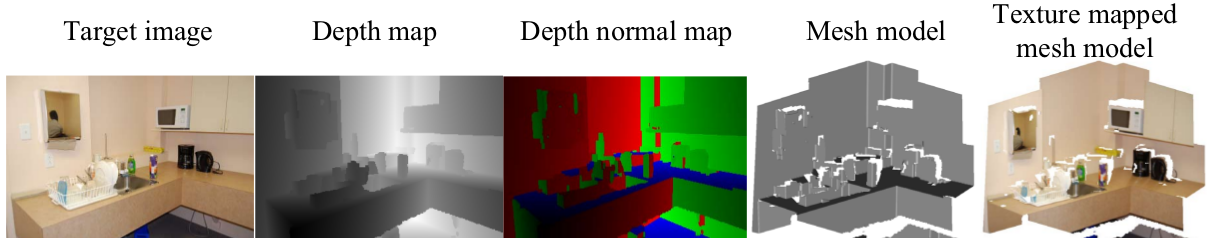
\includegraphics[width=1.0\textwidth]{img/depthmap}
 \caption{Pipeline of \FurukawaOld, including a typical depth map. Images taken from \cite{Furukawa2009}.}
 \label{fig:depthmap}
\end{figure}

Most algorithms are based on matching pixels based on a photo-consistency measure \cite{Seitz2006}. After rectification, only pixels on a particular line need to be tried. Those algorithms often use a prior promoting local smoothness, such as a Markov Random Field (MRF), while using a graph-cut algorithm to find a solution. The number of possible depths can be kept low, lowering the number of computations and increasing smoothness while allowing jumps in depth (\eg Figure \ref{fig:depthmap_layer}). Plane-sweeping algorithms iterate between assigning pixels to planes, and refining the plane equations. One fast but inaccurate plane-sweeping stereo algorithm is used by \Merrell2007 to quickly construct rough depth maps for further processing. Although the depth maps are imprecise, images can be processed very fast and depth maps are merged, obtaining reliable high-resolution dense point clouds. An example using an even stronger planar prior is the work by \FurukawaOld, who search for points with strong confidence depths and normals, and find three dominant axes that are more or less perpendicular. Hypothesis planes are proposed based on the points with strong confidence, and a MRF is used to assign pixels to hypothesis planes, obtaining a planar (Manhattan) world consisting of the most confident planes. Example images from their pipeline are shown in Fig. \ref{fig:depthmap}.

Although planes are a useful prior in indoor scenes and scenes with a lot of human-made architecture, the smoothness prior is more useful in natural environments (\ie general outdoor scenes). The approach of \Hernandez2007 uses photo-consistency in scene-space, whereby projection lines of pixels (\ie a set of possible depth locations) are projected onto camera planes nearby, and the depth candidates giving the best overall photo-consistency are picked. The estimated depths are then used in their carving algorithm using 3D graph-cut on a voxel grid.

Larger areas can be reconstructed using video and reliable location estimation (for example, using SLAM techniques). \Pollefeys2008 developed a system for real-time urban 3D reconstruction. It uses GPS and inertia sensors in addition to image-based pose estimation for reliable localisation, and uses a plane-sweeping dense stereo algorithm with a prior preferring locations containing points from the SfM sparse point cloud. Again, depth maps are created at a high rate and then merged into more accurate models. A similar large-scale reconstruction method is described by \Frahm2010. Building on the success of the Photo Tourism system \cite{Snavely2006} they collect publicly available images on the internet; however, large amounts of images make extensive matching of image pairs intractable, therefore their system finds clusters of images with use of their short image descriptor before structure from motion is applied. For each cluster, dense stereo is used and clusters are merged based on Geo-tag location and inter-connected clusters, finally obtaining a dense reconstruction for a big part of a city, within a day on a powerful PC.

% TODO maybe:
%     - Merging of depth maps (put somewhere logical)
%     - Surface reconstruction (+ multi-res paper)





%%%%%%%%%%%%%%%%% CONTENT: CONTRIBUTION %%%%%%%%%%%%%%%%% 
\chapter{Contribution} % / Design / ...
\label{contribution}
%\input{contribution.tex}


\chapter{Implementation}
\label{chp:impl}
%% IMPLEMENTATION

% - introduction
In this chapter, details on implementation of the proposed method are discussed. Code is listed in Appendix \ref{app:code}, supplied on DVD, and made available online\footnote{Code available on Google Code: http://code.google.com/p/martijn-msc-thesis}; this chapter will complement the code and will serve as a general introduction, therefore no code is listed in this chapter. The pipeline given in Section \ref{pipeline} will be used as a guideline, allowing the reader to follow the process in execution order. This order, though, is not necessarily the order of implementation; in fact, most applications developed for visualisation (last step in the pipeline) were written in an early stage, allowing for following progress and viewing intermediate steps. Developing geometry reconstruction algorithms greatly benefits from the ability to quickly shoot footage, run suggested and implemented algorithms, \emph{visualise} intermediate steps, and suggesting modified algorithms. Details on collecting datasets (first step in the pipeline) are discussed in the next chapter; implementation details of the remaining steps in the pipeline are discussed after an overview of the libraries that are being used.


% - libraries and external code
\section{Libraries}  \label{libraries}
All tools are written using platform-independent and open-source libraries, and all code should compile and run on all major platforms (although extensive tests have only been done under Linux, Ubuntu 12.04). The same holds for all tested external tools (SfM step), except Voodoo which is only free for research-purposes. All tools developed for this thesis are written in C++ and a cmake config file is provided.

The well-established computer vision library \textbf{OpenCV}\footnote{OpenCV homepage: http://opencv.willowgarage.com} \OpenCV is used for general image and video i/o, and 2D image and feature visualisation. Very recently, a sister project called \textbf{Point Cloud Library}\footnote{PCL homepage: http://pointclouds.org} (PCL) was announced by \Rusu2011, providing common data structures, algorithms, and tools useful for 3D computer vision. Although PCL still lacks extensive documentation and has a rapidly changing API, it does provide useful data structures and tools for handling point clouds, including advanced filter, segmentation and surface algorithms. Regrettably, it has (yet) no data structures for visibility information nor a commonly-agreed camera representation, reflecting the rare interest in visibility and occlusion (Sect. \ref{sfm}), so they have been developed for this thesis. In addition, the provided voxel grid representations are mostly useful for space partitioning and searching. Instead, we used the more suitable and feature-rich library \textbf{OctoMap}\footnote{OctoMap homepage: http://octomap.sourceforge.net}, recently released by \Wurm2010. OctoMap was chosen because it makes use of probabilistic nodes, implements a memory-efficient octree instead of same-size voxels, and allows for ray shooting. It also includes an octree viewer. Lastly, a set of open-source C++ files released by \Boykov2004 has been used for efficient graph-cut regularisation. Needless to say, writing methods to convert between representations of these four libraries was inevitable.


% - pipeline:
\section{Pipeline implementation}  \label{pipeline-implementation}

%   - SfM tools
\subsection{Structure from Motion}
Camera models and a feature point cloud can be obtained by standard Structure from Motion algorithms (Sect. \ref{sfm}). Structure from Motion has been implemented oftentimes already. Nowadays, reliable software tools are available for processing image sequences and outputting camera poses and point clouds. Both commercial and open-source tools exist. Since the proposed algorithms use SfM output as is and do not innovate on the SfM process itself, we experimented with three freely available Structure from Motion tools instead of building our own. The tools tested are Bundler, Voodoo, and VisualSfM. All tools are used with default settings.

Originating as part of the Photo Tourism work \cite{Snavely2006} and released under the GPL open-source license, \textbf{Bundler}\footnote{Bundler homepage: http://phototour.cs.washington.edu/bundler} became an authority and is still one of the most cited SfM systems. Originally developed for unordered photo collections taken from the internet, it claims to work on normal sequences too. The command line tool takes a directory with images as input, extracts and matches SIFT features and descriptors by default, and optimises estimated parameters incrementally using sparse bundle adjustment. Bundler outputs an ASCII file containing camera models, triangulated points with colours and visibility lists. The latest binary version (0.3) was tested.

\textbf{Voodoo}\footnote{Voodoo homepage: http://www.digilab.uni-hannover.de/docs/manual.html} was developed as non-commercial alternative to software tools such as Boujou and is free to use for research purposes. Finding and matching SIFT descriptors is possible, although by default Harris edge detection is used and points are tracked over the sequence. Voodoo is developed for sequences only for which the small displacement assumption is reasonable. The GUI allows for manually fine-tuning of estimated feature tracks (\eg linking a lost feature point to its rediscovery a few frames later) and includes simple modelling tools for improving the results, but those are not used during testing. Voodoo outputs various ASCII file formats, but unfortunately none of them includes visibility information. The latest version (1.2.0 beta) was tested.

Recently, a new graphical tool called \textbf{VisualSfM}\footnote{VisualSfM homepage: http://www.cs.washington.edu/homes/ccwu/vsfm/} by \Wu2011 was released that constitutes a graphical shell around a GPU implementation of both SIFT (SiftGPU) and Bundle Adjustment by \Wu2011 for SfM, and the CMVS/PMVS tools by \Furukawa2010 for patch-based dense multi-view stereo. VisualSfM and its components are all released under the GPL license. VisualSfM outputs an ASCII file similar to Bundler's format, and a binary file after the optional dense reconstruction step. The interface offers visual feedback during incremental bundle adjustment, and provides quite a few other useful visualisations. The latest version (0.5.17) was tested.

Example outputs are shown for two datasets; one example frame for each is pictured in Fig. \ref{fig:sfmcomparison0}). The chess dataset gives typical results and are shown in Figure \ref{fig:sfmcomparison1}; good results are obtained for the houses1 dataset, shown in Figure \ref{fig:sfmcomparison2}. More details on all datasets used in this thesis are listed in Appendix \ref{app:datasets}.

In general, Bundler performs poorly on the supplied datasets. Output usually consists of a point cloud without identifiable structures. An explanation for the bad results can lie in the fact that Bundler is developed for unordered sequences and therefore uses no prior for camera displacement nor for possible identical camera models. Indeed, estimated camera locations often have a variety of distances (and intrinsics) from the point cloud, where the other two tools place cameras in a string. Voodoo often exports reasonable results with, indeed, trustworthy looking camera paths and point clouds. It does not export colours and does not automatically rediscover points lost during tracking earlier on in the sequence, and no bundle adjustment is used to improve results. Using SIFT matching does not improve results, and matching only occurs between nearby frames. Voodoo results often contain a fair amount of points triangulated very far away from the scene. More importantly, none of the variety of export formats contains visibility lists. VisualSfM gives good results on almost all tested sequences. Due to its GPU implementation, it is faster than Bundler (and Voodoo in SIFT matching mode): two hours on sequences of 500 frames against half a night. Visual feedback during reconstruction and bundle adjustment is useful for monitoring progress. Due to Bundler's bad results, Voodoo's lack of visibility lists, and VisualSfM's good performance over all, VisualSfM is used for all further experiments.

\begin{figure}[htb!]
 \centering
 \subfigure[Frame 70 of chess dataset]{
  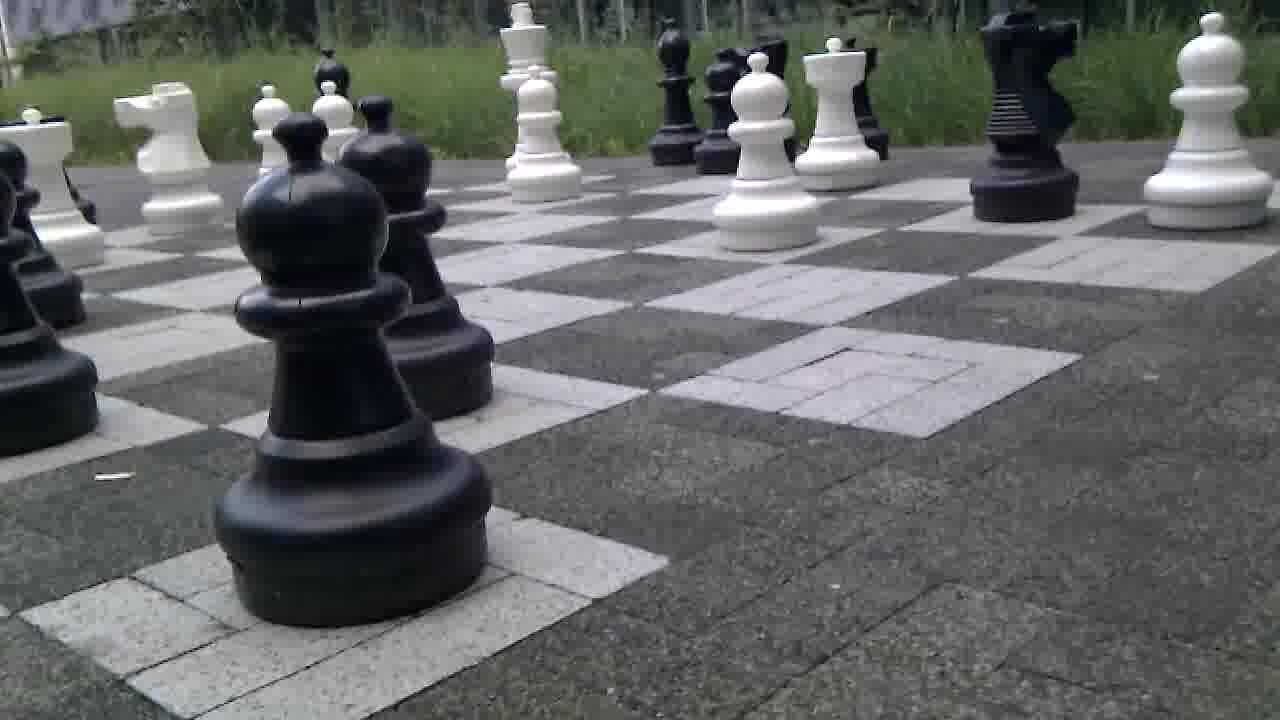
\includegraphics[width=0.55\textwidth]{img/chess_frame70}  \label{fig:}
 }
 \subfigure[Frame 11 of houses1 dataset]{
  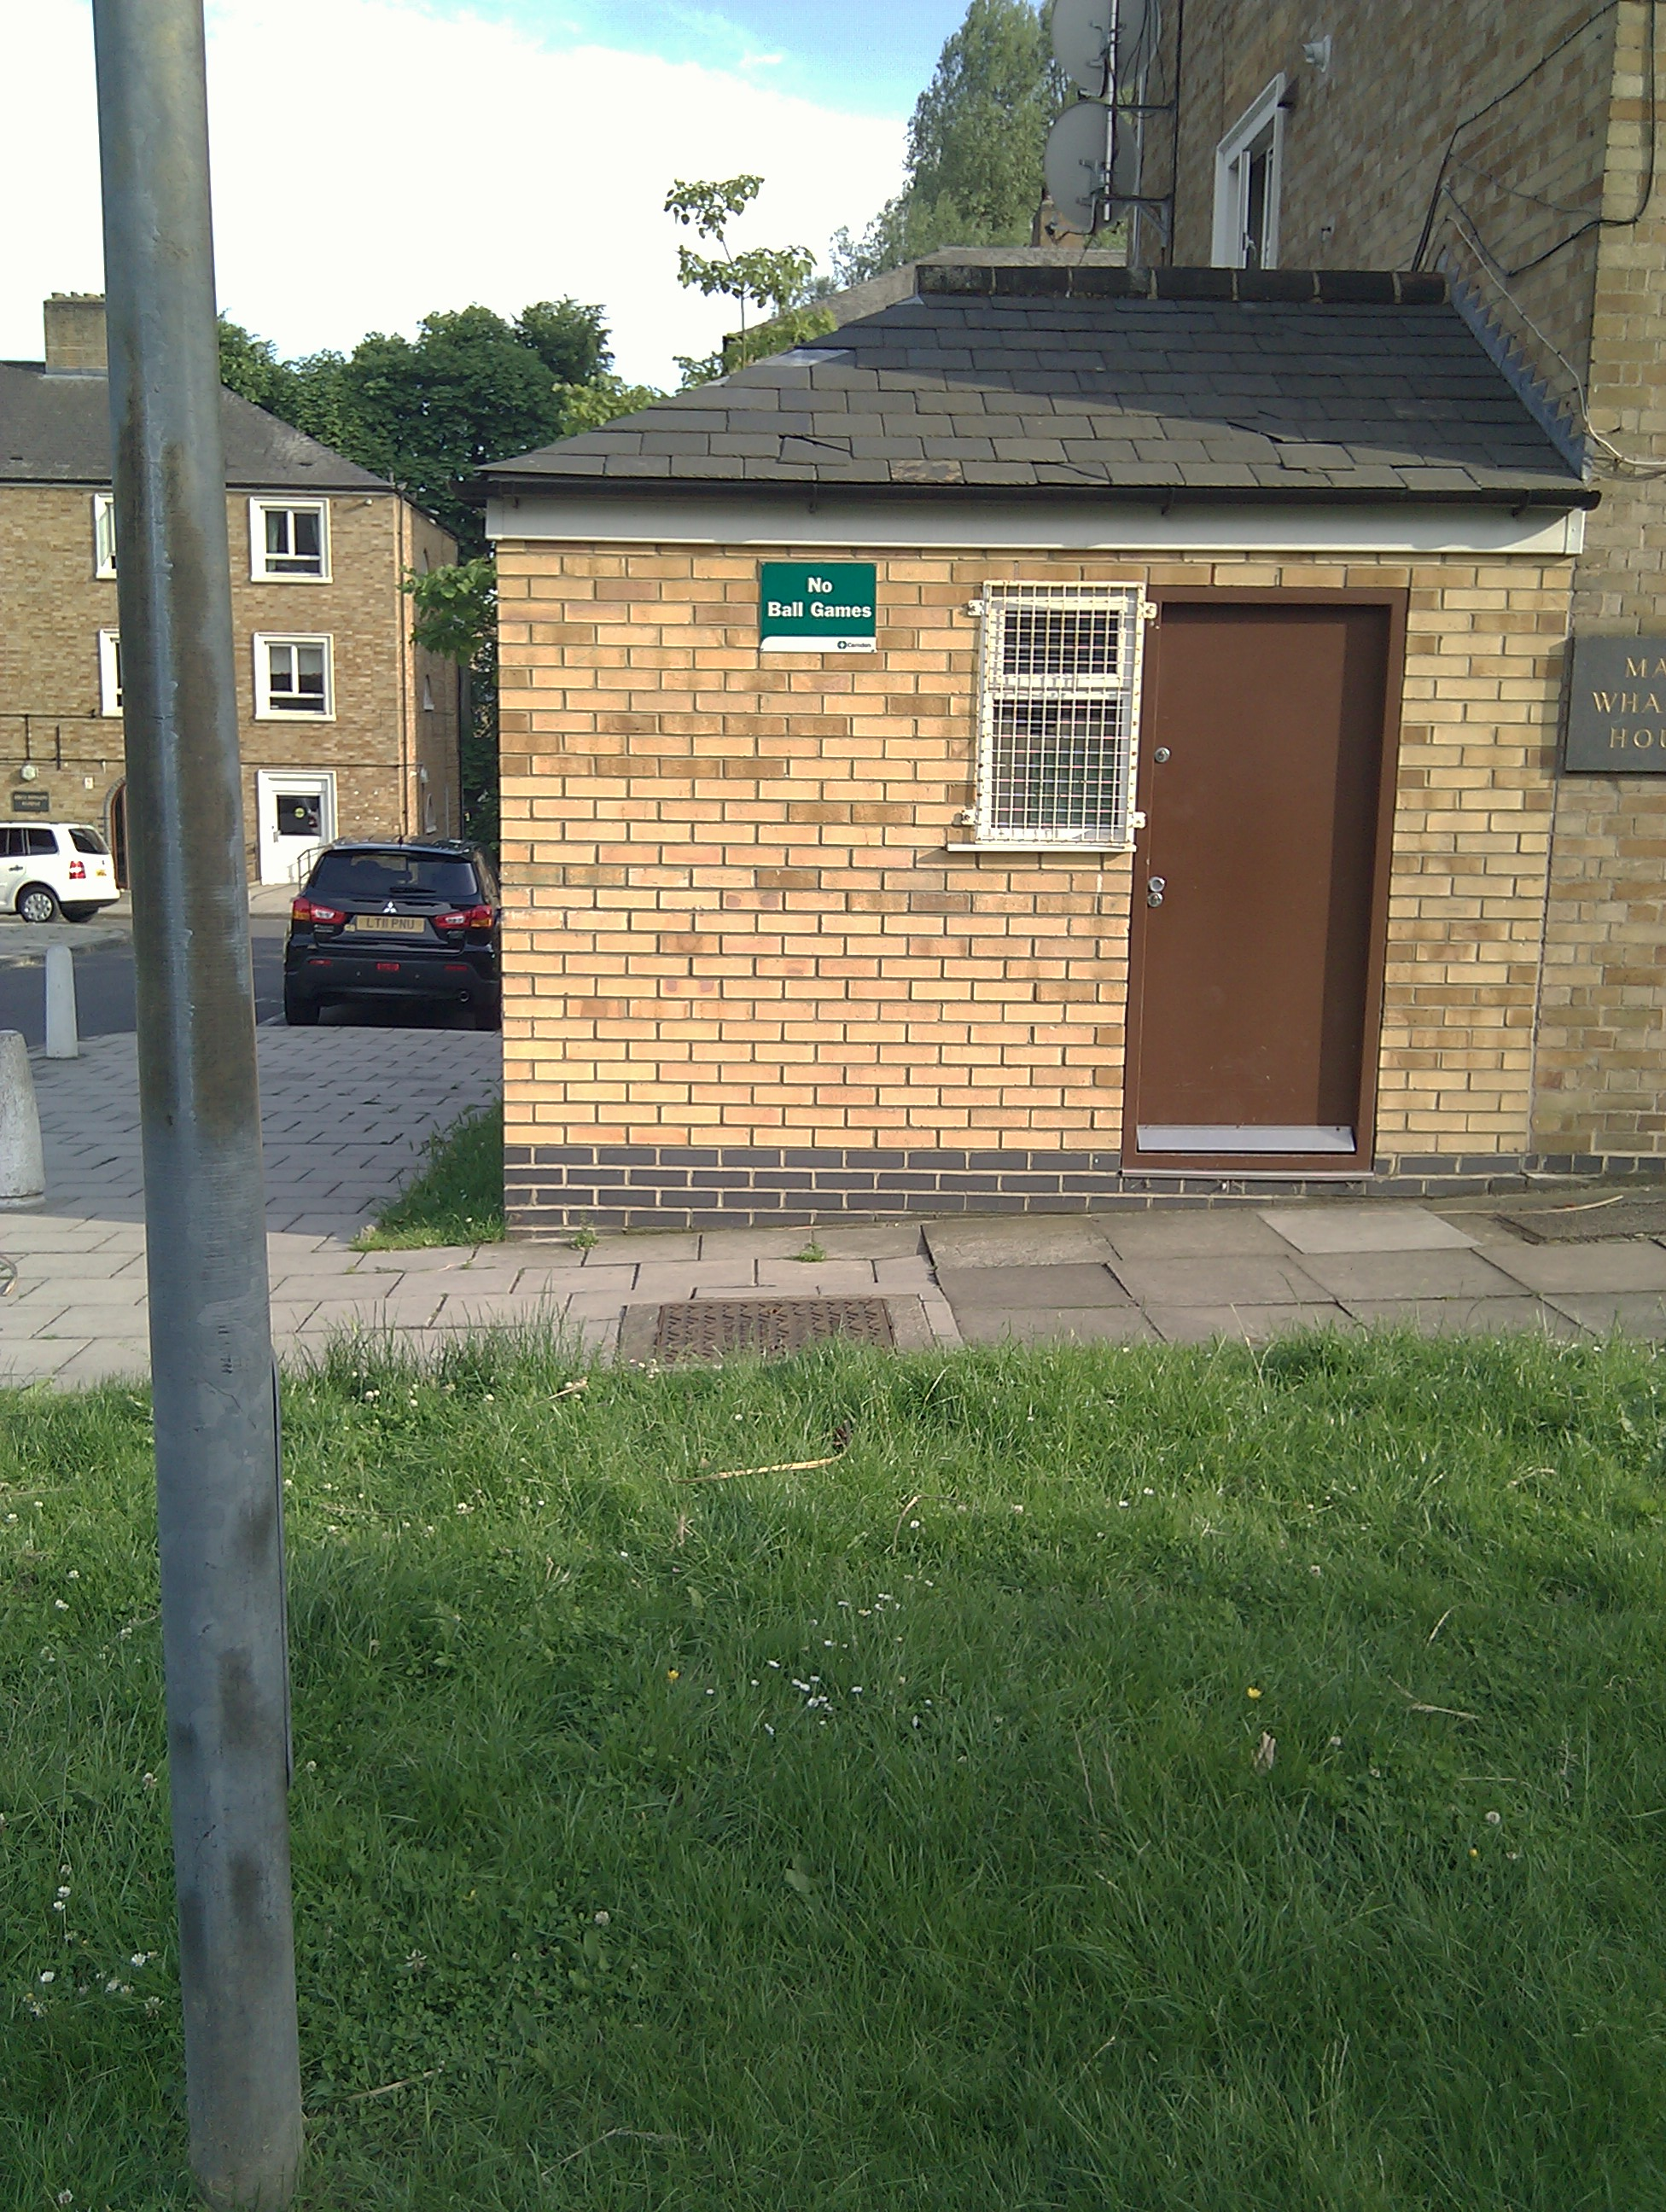
\includegraphics[width=0.35\textwidth]{img/houses1_frame11}  \label{fig:}
 }
 \caption{Example frames for chess and houses1 dataset (used for SfM tools comparison).}
 \label{fig:sfmcomparison0}
\end{figure}

\begin{figure}[htb!]
 \centering
 \subfigure[Bundler output]{
  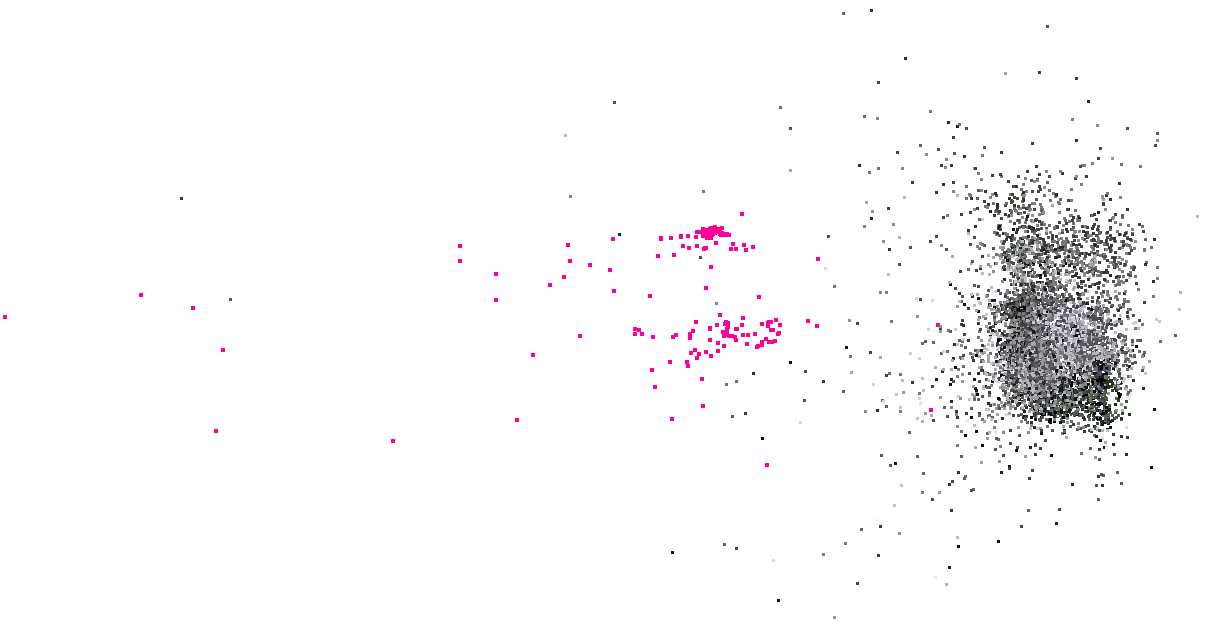
\includegraphics[width=0.9\textwidth]{img/chess_bundler}  \label{fig:}
 }
 \subfigure[Voodoo output]{
  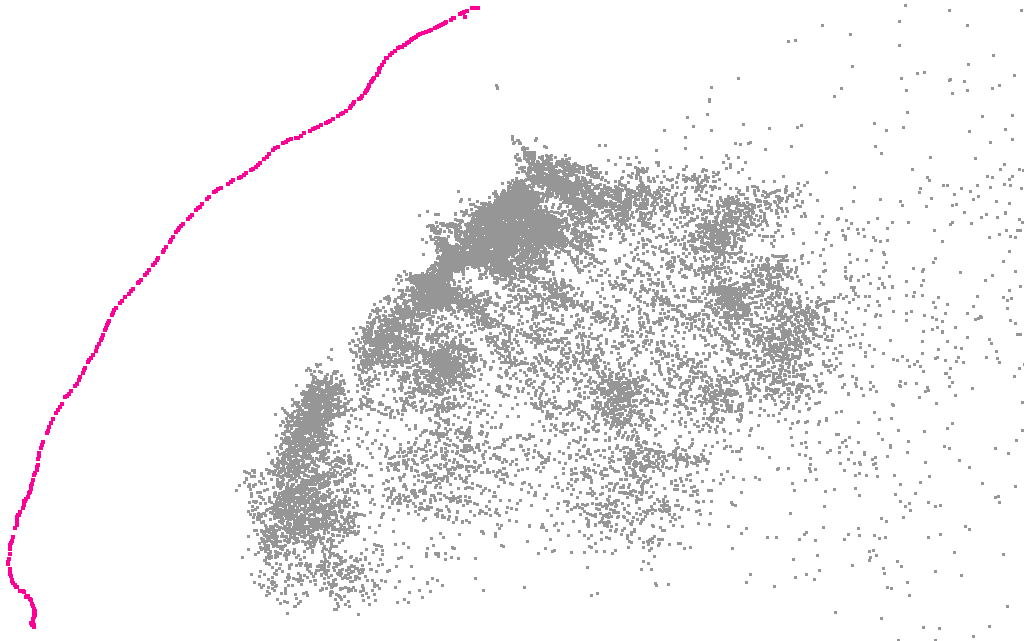
\includegraphics[width=0.9\textwidth]{img/chess_voodoo}  \label{fig:}
 }
 \subfigure[VisualSfM output]{
  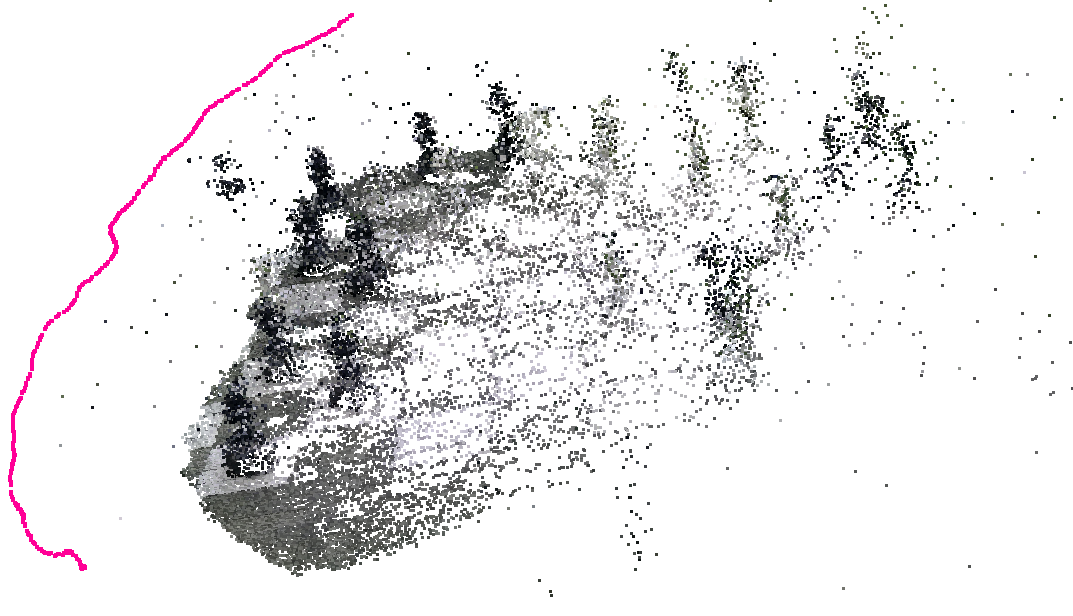
\includegraphics[width=0.9\textwidth]{img/chess_visualsfm}  \label{fig:}
 }
 \caption{Comparison of Structure from Motion tools Bundler, Voodoo and VisualSfM; typical example (chess dataset). Points shown in estimated colour (or grey if not given), camera poses displayed in pink. Visualisations by \texttt{sfmviewer}.}
 \label{fig:sfmcomparison1}
\end{figure}

\begin{figure}[htb!]
 \centering
 \subfigure[Bundler output]{
  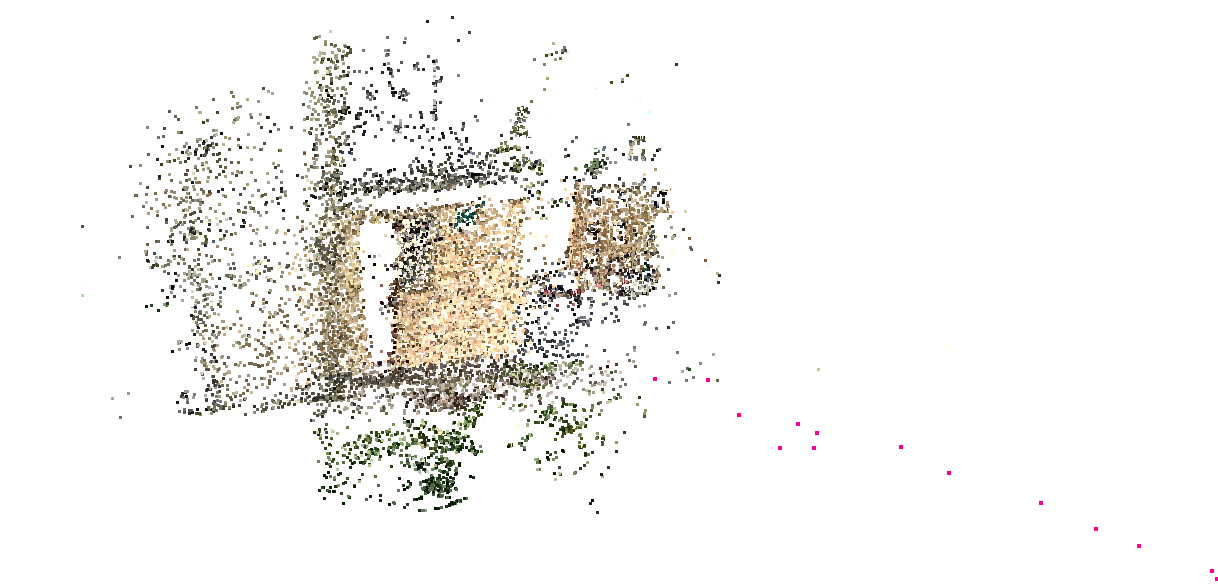
\includegraphics[width=0.9\textwidth]{img/houses1_bundler}  \label{fig:}
 }
 \subfigure[Voodoo output]{
  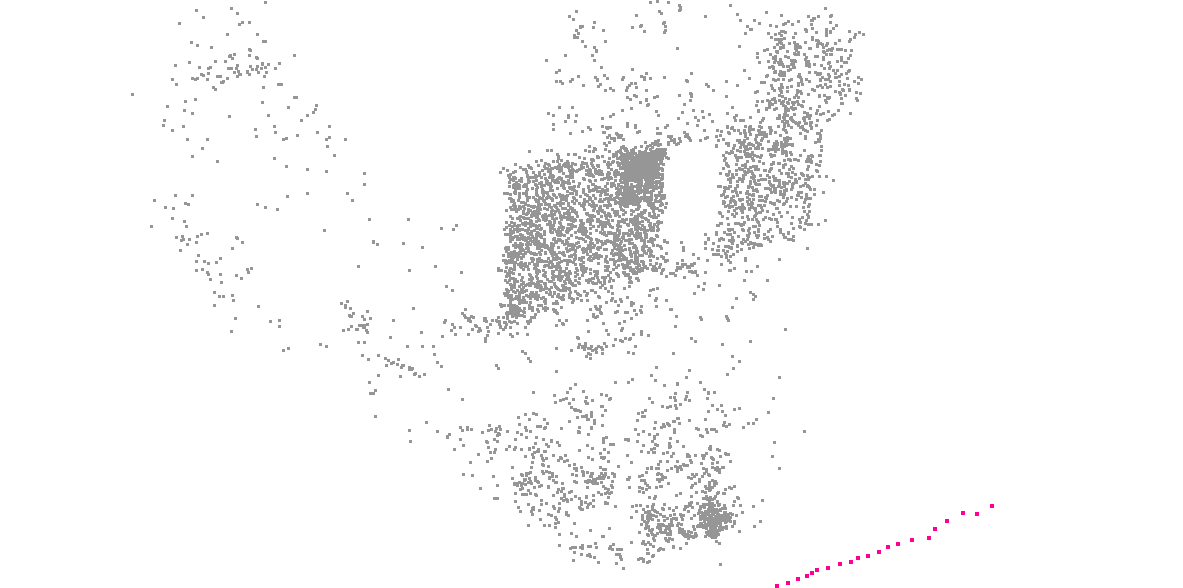
\includegraphics[width=0.9\textwidth]{img/houses1_voodoo}  \label{fig:}
 }
 \subfigure[VisualSfM output]{
  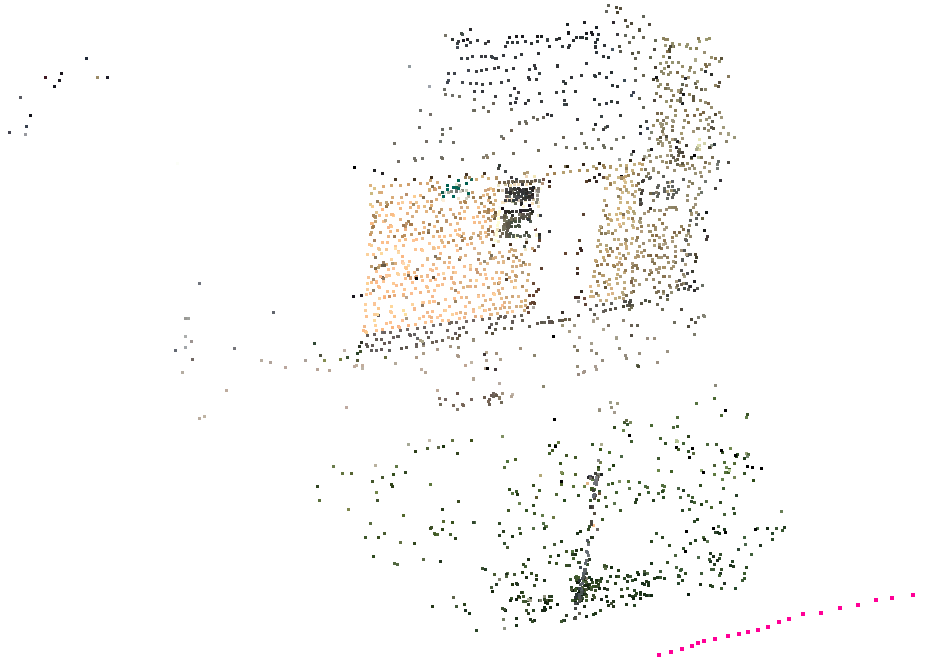
\includegraphics[width=0.9\textwidth]{img/houses1_visualsfm}  \label{fig:}
 }
 \caption{Comparison of Structure from Motion tools Bundler, Voodoo and VisualSfM. Good example (houses1 dataset). Points shown in estimated colour (or grey if not given), camera poses displayed in pink. Visualisations by \texttt{sfmviewer}.}
 \label{fig:sfmcomparison2}
\end{figure}

%   - (reading SfM tools output)
\clearpage
\subsubsection{Reading SfM output}
A common interface class \texttt{sfm\_reader} has been written for reading the various different formats used by different SfM tools. Furthermore, data structures from the C++ standard library are used to represent visibility information. Another reason to discuss this particular class is that it also provides useful methods for the carving algorithm concerning visibility and occlusion.

Four file formats parsers are written. The ply format (Stanford) is shared among SfM tools; however, it only contains points or polygon meshes. Ply files consist of a table (therefore, no variable length lists can be represented) and data can be binary or ASCII. The binary variant can be read by the PCL library, but for the ASCII data variant a parser has been written. Bundler and VisualSfM can both output the ASCII ply format, and VisualSfM outputs the binary ply format after dense reconstruction with CMVS/PMVS. Voodoo can output scripts for various programs (such as Blender). Its native output format has the common extension .txt and contains a list of points and a list of camera models.  Bundler's native output format has extension .out and contains camera models, points, and a visibility list for each point. VisualSfM's native output format has extension .nvm and contains the same information as Bundler's, although it contains a different camera model using quaternions instead of $R, t$ matrices, and distortion has one parameter instead of two. For all three native formats a parser have been written.

Points are saved in a \texttt{PointCloud} object as provided by PCL. It uses \texttt{PointXYZRGB} points which contain a location and an RGB colour. Cameras are saved in two separate structures: camera poses are saved in another \texttt{PointCloud} for easy visualisation - no pyramid-like camera visualisation wrappers are provided by PCL - as well as in a separate list of \texttt{camera} structures. The user-defined \texttt{camera} structure contains intrinsics $R$ and $t$, focal length, and two radial distortion parameters. All camera models from the different file formats are converted to this structure (\eg quaternion to $R$ matrix). Each visibility list is saved in a \texttt{std::map} object mapping every frame index for which a point was detected to a \texttt{visibility} structure. This user-defined structure contains the index of the feature for the particular frame, and the x and y coordinate of detection in the frame. Every feature point now has a global $(x,y,z)$ position in the \texttt{PointCloud} object, and a list of local $(x,y)$ camera coordinates for those cameras that detected the feature point. The map object allows for fast checks on visibility given a frame and feature point number, even for larger sets of frames.

Class \texttt{sfm\_reader} provides re-projection methods for given feature point and camera, including re-distortion. The method \texttt{reprojectsInsideImage} returns a boolean indicating whether a given point re-projects inside a camera window or not. This method is also used by \texttt{selectPointsForCamera}, which re-projects all points inside a given camera and makes an occlusion list of those points that could have been visible, but have not been detected (\ie the camera is not present in the visibility list). A list of currently visible points is made as well.

%   - (extending vis lists)
\subsection{Extending visibility lists}
The optional step of extending visibility lists checks all point-camera pairs that are not represented yet in the vector of maps of visibility information. In practise, this is implemented by looping through the points and, for each point, creating a visibility and invisibility list with help of the re-projection functions. Then, the whole sequence of a particular point is followed and all invisibility entries (re-projects inside image but not detected) are checked. The check consists of finding the nearest camera in absolute distance that did detect the feature point, re-projecting the point into that image and the current image, and comparing patches around the points. The size of the patches is determined by translating the feature point half the size of a voxel (given by the octree) in a direction perpendicular to the vector between the point and camera pose, re-projecting the translated point into one of the images, and calculating the distance to the projection of the original point. This distance is an approximation of the size of a projected voxel near the feature point, and is used to extract rectangular patches from the two images. They are compared by calculating the mean squared distance. A value below the threshold causes the camera index to be added to the visibility list of the feature point. By manually inspecting patch pairs and mean squared distance values, the threshold was set to 0.2 for all further experiments.

%   - carving
\subsection{Carving}
The proposed carving algorithms are implemented using the probabilistic octree of the OctoMap library \cite{Wurm2010}. The octree is initialised with a single parameter specifying the smallest node size possible. By default, all ray shooting operations are executed on nodes at this smallest scale, that is, the leaf nodes in the tree representation. Various node types are provided, the one containing probabilities is used. Probabilities are stored logarithmically, but conversion to and from normal probability values is straight-forward. Two thresholds are used to allow nodes to be labelled with either `free' ($val <= Thr_{free}$) or `occupied' ($val >= Thr_{occ}$), or no label (unknown). Those thresholds are $Thr_{free} = 0.2$ and $Thr_{occ} = 0.7$ by default, and are kept at these values for all experiments. For memory efficiency, eight (leaf) nodes can be merged recursively if they have the same label, thereby averaging and thus losing individual occupancy probabilities. By default leaf nodes are not initialised and depth of the tree is kept to a minimum.

For the implemented space carving algorithms, the octree is initialised with smallest node size equal to the largest axis variation in the feature point \texttt{PointCloud} divided by a given resolution parameter. OctoMap provides two ray shooting methods: \texttt{computeRayKeys} takes as input two points and returns a list of node keys that were hit by the ray between the two points; \texttt{insertRay} does the same, but sets the last node to $Thr_{occ}$ and all the others to $Thr_{free}$ instead of returning the list. The latter is used for the binary Visibility Space Carving algorithm (Alg. \ref{alg:vis-carving}), and the former is used for both probabilistic Visibility-Occlusion Space Carving algorithms (Alg. \ref{alg:vis-occ-carving} and \ref{alg:vis-occ-carving-veto}), there where \texttt{getVoxelsBetween} is mentioned. Note that since we carve tubes of space in this implementation, the resolution parameter potentially has a big influence on the result. In practise, there is a range of possible resolution values that give good results, and the range is laid down by the dataset provided.

%   - regularisation
\subsection{Regularisation}
Regularisation is implemented used the code provided by \Boykov2004. For simplicity, the octree is converted to a voxel grid with voxels the size of the smallest possible octree node. First an empty voxel grid is initialised using the occupancy prior for unknown space, which we set to $Thr_{unknown} = 0.2$. Since conversion splits existing bigger nodes and adds nodes where nothing was initialised before, this increases memory usage quite a lot. This means that only lower resolution settings can be used in the regularisation process. After applying the graph-cut algorithm the voxel grid is converted back to the memory-efficient octree representation.

%   - visualisation/viewers:
\subsection{Visualisation}
During the pipeline, a few intermediate and final results can be visualised. Three visualisation tools are developed and one provided by the OctoMap library is used. We will discuss each briefly. The first two tools are used for visualising features before carving, one 2D image annotator and one interactive 3D tool. The two other tools are meant for visualising voxel grids after carving, again one 2D image annotator and one interactive 3D tool.

%     - features (annotated imgs)
Although external structure from motion tools are being used, a tool has been written for experiments with and visualisations of various feature detectors. It can be used to check the amount of interest points discoverable in a dataset, and the uniqueness of their descriptors during tracking. It is not used in the final pipeline, but is discussed for completeness. The visualiser, \texttt{featureviewer}, takes as input either a video, directory with images, or webcam stream, and annotates the images with a given type of interest point (\eg SIFT, SURF, ORB, FAST, HARRIS) including their size, plus edges (Canny edge-detector). One can interactively click on a feature point, which will be matched over the sequence by a simple ratio test: if the ratio of the two best matches in the next or previous frame (\ie the L1 distance) is big, the interest point is quite unique and the best match is taken. If the ratio is close to 1, we keep the last known good descriptor and continue to the next frame. Note that this simple heuristic does not use any location prior. We can define the visibility confidence as one minus that ratio, and plot it for the sequence, similar to the visibility tracks shown in Fig. \ref{fig:vis-carving} and \ref{fig:vis-occ-carving}. One example image processed with \texttt{featureviewer} is shown in Figure \ref{fig:featureviewer}.

%     - sfm (3D)
Visualisation of triangulated SfM feature points or dense point clouds can be done with \texttt{sfmviewer}. The SfM tools outputs (Fig. \ref{fig:sfmcomparison1} and \ref{fig:sfmcomparison2}) were made this way. It uses class \texttt{sfm\_reader} for opening SfM output files and representing their contents. The PCL library provides wrappers around the VTK visualisation toolkit. It is used for easy point cloud visualisation, both the feature point cloud and camera poses. Interaction is implemented using the default PCL visualiser for mouse navigation, plus VTK call-back functions for custom shortcuts, and selection of points and cameras. Selecting a point colours the cameras that detected the point (using the visibility list of the point). Selecting a camera calls \texttt{selectPointsForCamera} as described earlier, thereby projecting all the points into the camera. Detected points are coloured green, while undetected points that do re-project within the image borders but are coloured red. To be able to recover the original point colours during the next selection, \texttt{sfm\_reader} keeps a shadow copy of the original point cloud. Another implemented feature is the ability to visualise those visible (green) and invisible (red) points onto the original corresponding frame. The camera-feature pairs can be visualised even more explicitly by drawing green lines between the camera and visible points or between the point and detecting cameras. Two example visualisation is shown in Fig. \ref{fig:sfmviewer1} and \ref{fig:sfmviewer2}.

\begin{figure}[htb!]
 \centering
 \subfigure[\texttt{featureviewer} for frame in chess, including SIFT features and visibility track for the green interest point]{
  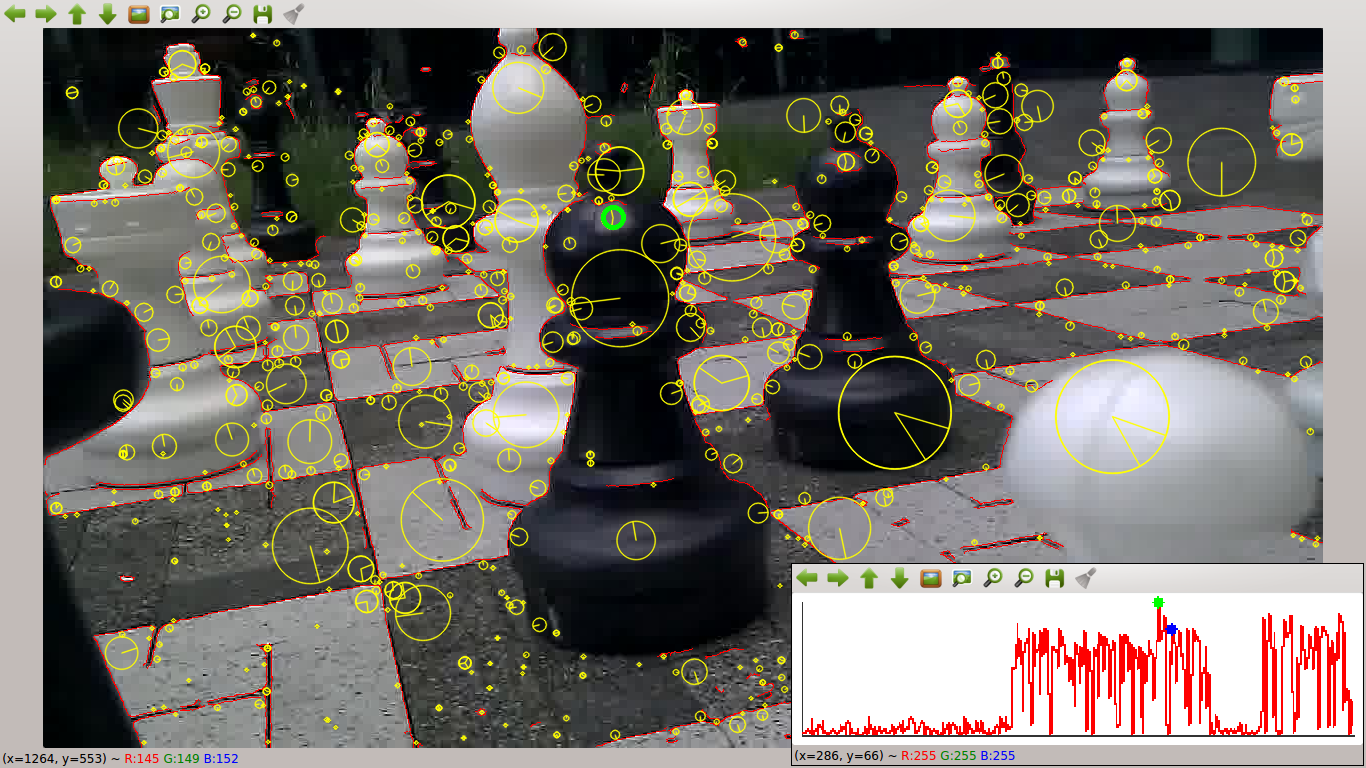
\includegraphics[width=0.9\textwidth]{img/featureviewer}  \label{fig:featureviewer}
 }
 \subfigure[\texttt{sfmviewer} for selected camera of lampposts\_on\_wall1; one lamppost causes a red area to emerge on the wall, but the conservative visibility information of VisualSfM is noticeable too in the `green' areas]{
  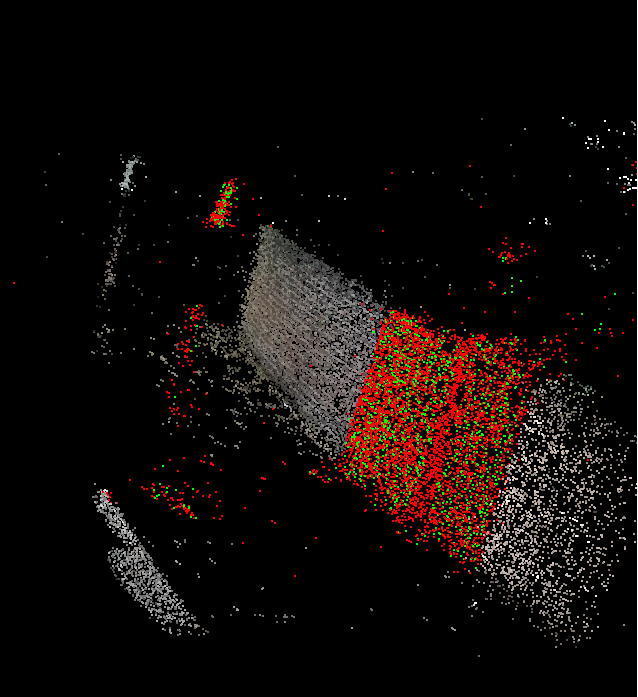
\includegraphics[width=0.45\textwidth]{img/sfmviewer2}  \label{fig:sfmviewer1}
 }
 \subfigure[\texttt{sfmviewer} for selected point of sainsburys1; two reflective poles become `visible' due to absence of lines]{
  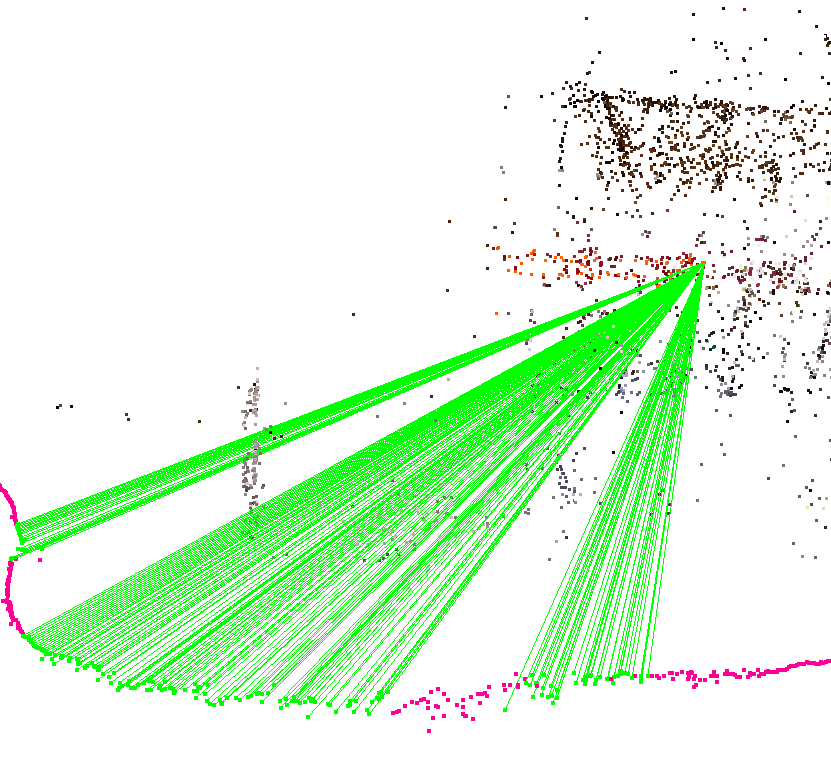
\includegraphics[width=0.45\textwidth]{img/sfmviewer1}  \label{fig:sfmviewer2}
 }
 \subfigure[\texttt{carveviewer} for frame in sciencepark2 (with incorrect nearby voxels at the top and only few detected features)]{
  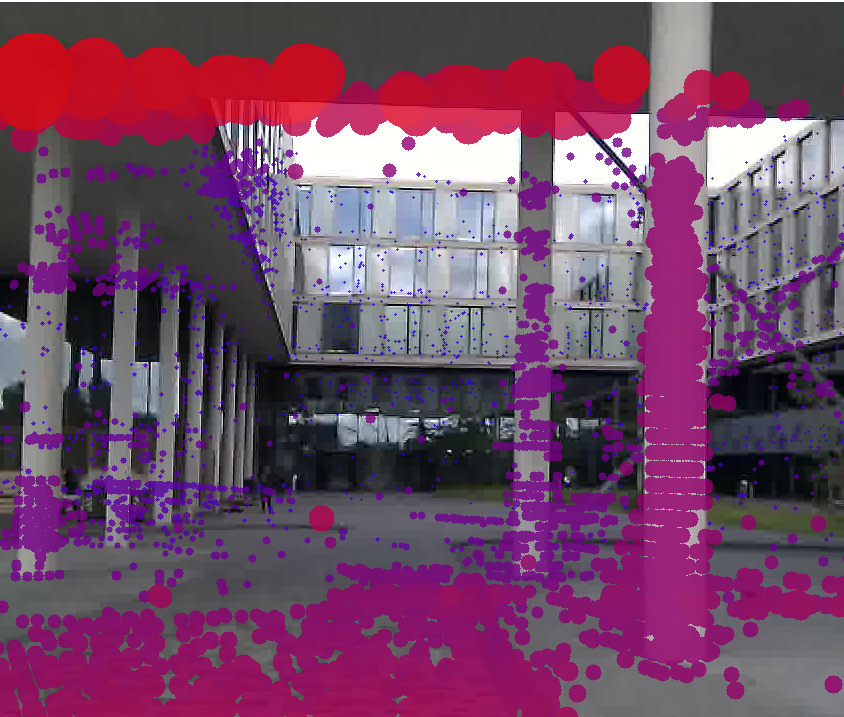
\includegraphics[width=0.45\textwidth]{img/carveviewer}  \label{fig:carveviewer}
 }
 \subfigure[\texttt{octovis} view for houses1; a partly reconstructed lamppost is visible on the left (purple)]{
  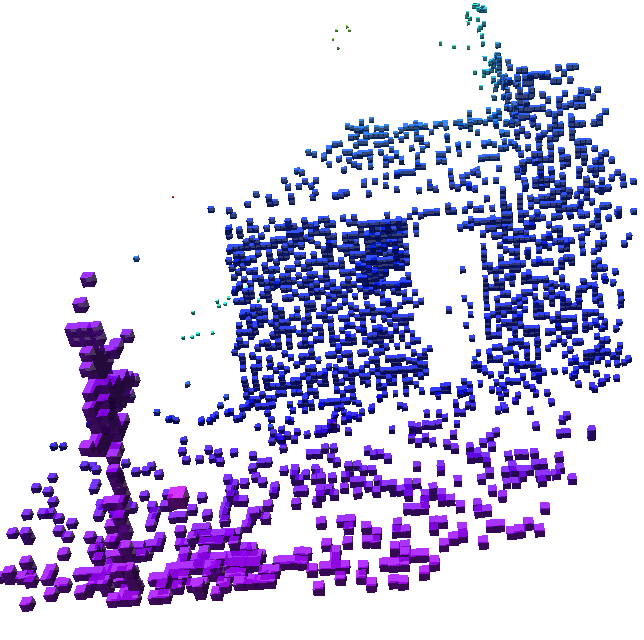
\includegraphics[width=0.45\textwidth]{img/octovis}  \label{fig:octovis}
 }
 \caption{Visualisations by three developed tools and one provided viewer}
 \label{fig:visualisationtools}
\end{figure}

\clearpage
%     - carveviewer (annotated imgs)
After space carving has been done, a probabilistic octree is the result. For visualisation purposes, we use the occupancy threshold $Thr_{occ}$ to make a binary distinction between occupied and not occupied. The last developed visualisation tool, \texttt{carveviewer}, annotates the original images with the carved octree. To prevent axis dependent results, all nodes are imagined as spheres and projected on top of the images. As with the code for extending visibility lists, both the node centres and centres with offsets the size of the nodes are projected into the images, and the projected points are used to estimate the radii, resulting in a list of $x,y,r$ entries. Then, rays are casted from the camera in the direction of the projected nodes, and all rays hitting another, occluding node before the projected one, are removed from the list. The remaining nodes are visible from the given camera and are drawn as semi-transparent circles on top of the image. The circles are drawn with the estimated radii and coloured according to the log distance from the camera (nearby voxels are red, voxels far away blue). One example rendering is shown in Figure \ref{fig:carveviewer}. For more dense voxel grids, results remind of depth maps on top of their original images. 

%     - octovis (3D)
An interactive octree viewer is provided by the OctoMap library. It has been used without modification. Nodes are rendered as semi-transparent cubes which are either light blue for occupied and dark blue for very high occupancy probability (threshold undefined), or coloured according to the value of one of the axes. Optionally, free space (occupancy probability below $Thr_{free}$) can be visualised too as green cubes. One example view is shown in Figure \ref{fig:octovis}.

The visualisation tools will be used extensively in the next chapter.







Equations can be inserted either within the text as $x=\phi/2$, or preferably, as
numbered equations where

\begin{equation} \label{myEqName}
 p(\mathbf{Z}_{k}|\mathcal{T}_{k},\mathbf{e}) = \prod_{i\in S_{k}}
G_{z_{i,k}}[\mu_{\mathcal{T}_{k}(i)},\phi_{\mathcal{T}_{k}(i)}],
\end{equation}

and the equation still receives proper punctuation because equations are just normal parts of sentences.

You can reference the above equations like this:  Equation~\ref{myEqName}, or (\ref{myEqName}) for short.  You can also reference sections:  Section~\ref{sectionExample}. Notice that in the .tex file, one can precede \texttt{$\backslash$ref} with a tilde ($\sim$). Using a tilde instead of a space forces a small space to happen there, and essentially glues the previous word to the label being referenced. This keeps a line-break from interrupting your reference like this: Equation\\ \ref{myEqName}. 

One should cite papers by referring to the only author, or the only two authors together, or to just the first author if there are three or more.  So one may say that we gained great wisdom from Weiss~\cite{WeissICCV01}, have been enlightened by Tuytelaars and Van Gool~\cite{TuytelaarsCVPR.2004:SynchVideo}, and are inspired by Vedula~\etal~\cite{Vedula:2005:ISM}.






%%%%%%%%%%%%%%%%% EVALUTATION %%%%%%%%%%%%%%%%% 

\chapter{Results and Evaluation}
\label{chp:eval}
%\input{evaluation.tex}

\section{Figures} \label{sectionExample}


\chapter{Discussion and Future Work}
\label{chp:eval}
%\input{discussion.tex}




%%%%%%%%%%%%%%%%% CONCLUSION %%%%%%%%%%%%%%%%% 

\chapter{Conclusion}
\label{chp:conc}
%%% Conclusion

% general geometry reconstr + visibility info
The problem of geometry reconstruction is challenging and the diversity in scenes asks for solid solutions. The literature on geometry reconstruction is comprehensive and many approaches have been tried, with varying degrees of success. Most approaches are based on some form of photo-consistency, that is, they rely on \emph{directly} observing all objects that are being reconstructed. However, this casts constraints on the surface properties of the objects. Surfaces often need to be either uniformly coloured (low-textured) and well differentiable from the background, or they need to have clear and rich textures and Lambertian-like properties. In practice, these constraints are not always met. Therefore, many algorithms fail on certain kinds of objects.

% proposed algorithm
We proposed a new approach based on \emph{indirectly} observing objects using visibility information. Based on the intuition that detection of features from certain view points and absence of detection in others can provide clues on where occluder objects may exist, we developed two algorithms; one based on visibility information alone, and one using both visibility and occlusion (\ie absence of visibility). An occupancy grid is altered iteratively based on this information. Feature estimation is obtained by using reliable Structure from Motion tools and no pixel pair-wise guesswork needs to be done.

% results + comments / conclusion
The proposed method has been shown to provide reasonable results for scenes containing low-textured or reflective objects. For good results, enough view points need to be provided (\eg by walking around an object) and background objects containing a decent amount of features need to be present. Visibility information helps carving much of the empty space for which reliable features on background objects are extracted, but leaves space with less visibility rays partly labelled as occupied. Using both visibility and occlusion cues (and default world view `unknown') improves results, even though visibility information exported by standard structure from motion tools is often very conservative, making the majority of the occlusion claims untrue. Furthermore, the veto version of the Visibility-Occlusion algorithm (Alg. \ref{alg:vis-occ-carving-veto}) outperforms the recent dense reconstruction algorithm CMVS/PMVS on the tested reflective objects. Visibility and occlusion therefore appear promising cues for further research on geometry reconstruction. 

% future work
While sparse point clouds reconstructed by structure from motion are reliable, points do not have a clear size or shape and the exact shape of the affected space between cameras and features is therefore undefined. The taken approach of ray shooting and altering the tube of voxels hit by the ray makes the algorithm dependent on the amount of strong feature points and chosen resolution. In other words, the amount of features determines the maximum resolution. Future work could focus on relaxing those dependencies - allowing arbitrary voxel grid resolutions - by using features with better defined sizes. One possibility is to create features based on the provided sparse point cloud. For example, nearby and planar feature points can be combined to form local patches with known size and normal. They could be texture-mapped, projected into, and matched over the sequence. Potentially, small patches could also be combined using a graph-like connection map, and the changing graph over the sequence could be used for carving. The local patches could be seen as acting like small local `green screens' in the scene carving away part of space while the camera moves around.

Other features could be used as well. Edges could provide useful cues on object borders (\eg feature points disappearing after `hitting' an edge). As a last possibility, one could consider using full resolution occlusion images, for example using occlusion posterior predictions as given by the system of \Humayun2011 (for example outputs on our sequences, see Fig. \ref{fig:learningocclusions}). Hereby full-resolution probabilistic \emph{carve images} will be used instead of only a few sparse interest points. A solution needs to be found for the lack of depth, \ie where to stop carving.

Furthermore, texture mapping would make results more appealing and increases photo-realism, even for new (unseen) camera poses.

Lastly, we like to remind the reader of the observation that all current approaches - including the one proposed in this thesis - have both success stories and failure cases, but not necessarily the same failures. Therefore, the proposed approach may be used in conjunction with other approaches. For example, Visibility-Occlusion Space Carving can provide a fast and rough geometry reconstruction, which can be used as a prior for possible depths in patch-based or plane-sweeping multi-view dense reconstruction approaches.

\begin{figure}[htb!]
 \centering
 \subfigure[Frame from lampposts\_on\_wall1]{
  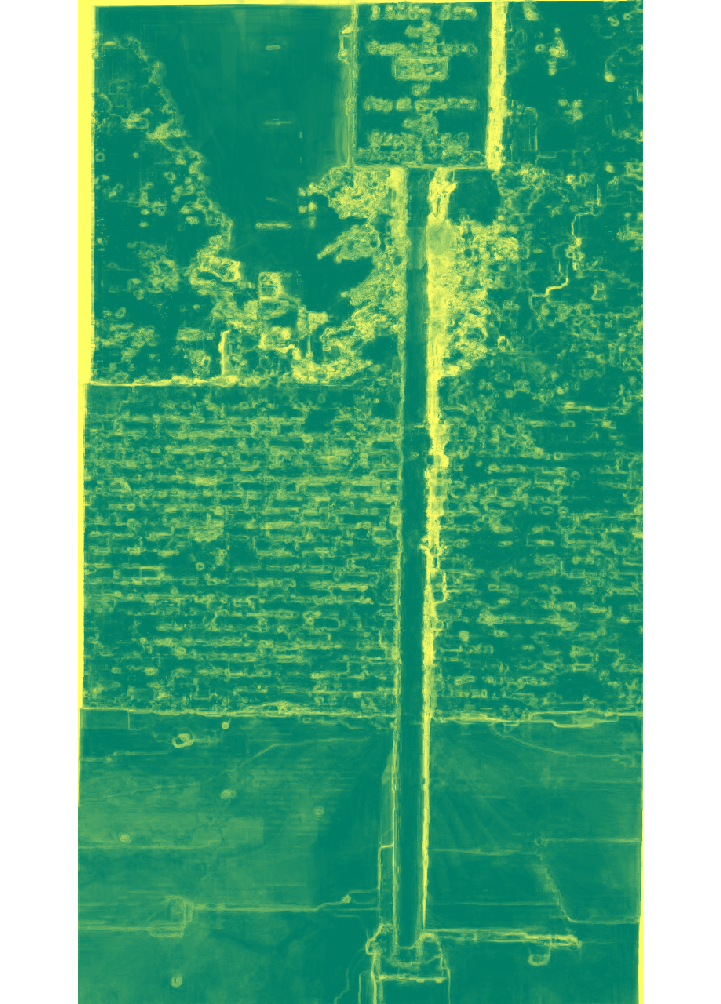
\includegraphics[width=0.35\textwidth]{img/learningocclusions1}  %\label{fig:}
 }
 \subfigure[Frame from houses1]{
  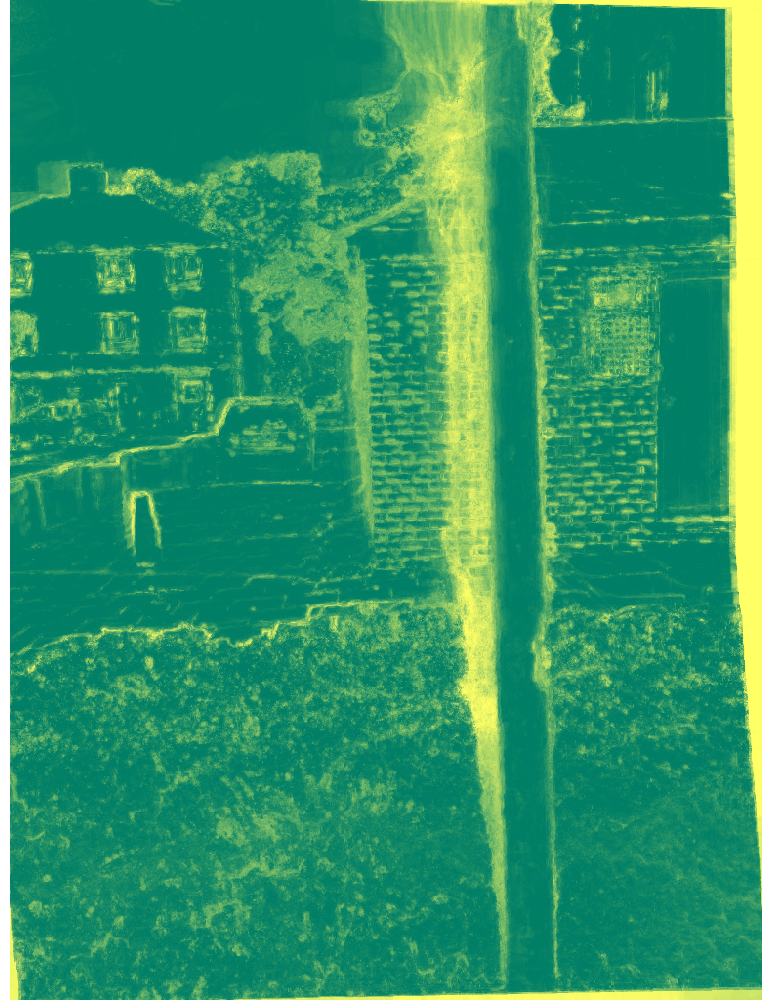
\includegraphics[width=0.35\textwidth]{img/learningocclusions2}  %\label{fig:}
 }
 \caption{Example output of the system developed by \Humayun2011, showing cyan for low and yellow for high probabilities of pixels getting occluded in the next frame}
 \label{fig:learningocclusions}
\end{figure}



\begin{figure}
\begin{center}
\begin{tabular}{c|cc}   % The "|" bar puts a bar in the figure
   \includegraphics[width=.30\columnwidth]{home.png} &  % The little "and" puts splits in the table
   \includegraphics[width=.30\columnwidth]{home.png} &  
   \includegraphics[width=.30\columnwidth]{home.png}\\
   (A) & (B) & (C)
\end{tabular}
\caption{Another figure caption. These should be meaningful and somewhat self-contained.} 
  \label{fig:SomeMoreFigs}
\end{center}
\end{figure}

Figures need not be in \texttt{.pdf} format. For example, Figure~\ref{fig:SomeMoreFigs} pulls in $3$ copies of a \texttt{.png} file. Also, notice that the automatic-placement of figures will try to put each figure as close as possible to the first reference in the final document, regardless of figure-placement in the .tex.




%%%%%%%%%%%%%%%%% APPENDICES %%%%%%%%%%%%%%%%% 

\addcontentsline{toc}{chapter}{Appendices}

\cleardoublepage
\appendix
\chapter{Theoretical Background}
\label{chp:theory}
%\input{theory.tex}

\chapter{Lisp Primer}
\label{cha:lisp-primer}
\input{lisp-primer.tex}




%%%%%%%%%%%%%%%%% REFERENCES %%%%%%%%%%%%%%%%% 

\addcontentsline{toc}{chapter}{Bibliography}

\bibliography{mscthesis}


\end{document}

